% SIAM Article Template
\documentclass[review,onefignum,onetabnum]{siamart171218}

% Information that is shared between the article and the supplement
% (title and author information, macros, packages, etc.) goes into
% ex_shared.tex. If there is no supplement, this file can be included
% directly.
% SIAM Shared Information Template
% This is information that is shared between the main document and any
% supplement. If no supplement is required, then this information can
% be included directly in the main document.


% Packages and macros go here
%\usepackage{natbib}
\usepackage{amsfonts}
\usepackage{graphicx}
\usepackage{epstopdf}
\usepackage{algorithmic}
\usepackage{siunitx}
\ifpdf
  \DeclareGraphicsExtensions{.eps,.pdf,.png,.jpg}
\else
  \DeclareGraphicsExtensions{.eps}
\fi

% Add a serial/Oxford comma by default.
\newcommand{\creflastconjunction}{, and~}

% Used for creating new theorem and remark environments
\newsiamremark{remark}{Remark}
\newsiamremark{hypothesis}{Hypothesis}
\crefname{hypothesis}{Hypothesis}{Hypotheses}
\newsiamthm{claim}{Claim}

% Sets running headers as well as PDF title and authors
\headers{FVM for 1-D Elastic Wave Equation}{A. Nolan}

% Title. If the supplement option is on, then "Supplementary Material"
% is automatically inserted before the title.
\title{An introduction to the finite volume method using the elastic wave equation 
\thanks{Submitted on 12/02/2019}}

% Authors: full names plus addresses.
\author{Andrew Nolan\thanks{\email{anolan@sfu.ca}}}

\usepackage{amsopn}
\DeclareMathOperator{\diag}{diag}


%% Added on Overleaf: enabling xr
\makeatletter
\newcommand*{\addFileDependency}[1]{% argument=file name and extension
  \typeout{(#1)}% latexmk will find this if $recorder=0 (however, in that case, it will ignore #1 if it is a .aux or .pdf file etc and it exists! if it doesn't exist, it will appear in the list of dependents regardless)
  \@addtofilelist{#1}% if you want it to appear in \listfiles, not really necessary and latexmk doesn't use this
  \IfFileExists{#1}{}{\typeout{No file #1.}}% latexmk will find this message if #1 doesn't exist (yet)
}
\makeatother

\newcommand*{\myexternaldocument}[1]{%
    \externaldocument{#1}%
    \addFileDependency{#1.tex}%
    \addFileDependency{#1.aux}%
}

% Optional PDF information
\ifpdf
\hypersetup{
  pdftitle={Linear Algebra and Adaptive Mesh Refinement},
  pdfauthor={A. Nolan}
}
\fi

% The next statement enables references to information in the
% supplement. See the xr-hyperref package for details.

%% Use \myexternaldocument on Overleaf
%\myexternaldocument{ex_supplement}

\begin{document}

\maketitle

% REQUIRED
\begin{abstract}
    An introductory description of finite volume methods for solving partial differential equations is discussed below. Conservation laws, the finite volume method, and the Riemann problem are all investigated via the one-dimensional elastic wave equation. We use the method of characteristic to reduce this couple set of equations too the advection equation which we the solve numerically via finite volume methods.
\end{abstract}

% REQUIRED
\begin{keywords}
  Finite Volume, PyClaw, Elastic Wave Equation
\end{keywords}

% REQUIRED
% \begin{AMS}
%   68Q25, 68R10, 68U05
% \end{AMS}

\section{Introduction} 
Numerical methods for solving partial differential equations (PDEs) arise across all scientific fields. From modeling future predictions of global sea-level rise to heat flow through a rod, numerical solution to PDEs at the heart of modeling physical phenomena. The finite difference method, which approximates derivatives using the Taylor expansion, is a common starting point for numerical solutions to PDEs. By using the Taylor expansion ordinary differential equations or PDEs can be reduced to a series of algebraic statements for which matrix methods can be used to solve efficiently.  

While the finite difference methods are a powerful starting point they have their limitations; one of which is dealing with discontinues. Due to the failure of the finite difference method and other numerical methods to deal with discontinuities, the finite volume method arises. The finite volume method is commonly used to solve hyperbolic PDEs, due to their susceptibility to developing shock waves, but can be used to solve all type of PDE. At the heart of the finite volume method is the \textit{Riemann Problem}, an initial value problem with piecewise constant initial conditions that naturally arises due to the discretized domain on which the equations are solved. 

We begin with an introduction to conservation laws and the finite volume method as motivated by the one-dimensional advection equation. We derive conservation laws based on physical intuition of fluid flow as guided by  \cite{leveque_2002}. We then use the conservative form of the advection equation to derive the finite volume method. First and second-order numerical flux approximation methods are stated. We also investigate higher-order slope-limiters through the 
\texttt{PyClaw} package. We then derive an analytical solution to the homogeneous (\textit{i.e.} constant-coefficient) elastic wave equation through the method of characteristics that we use to validate our numerical methods. Numerical experiments are conducted to investigate the performance of the numerical methods outlined. The code for the numerical experiments animations of the model runs can be found \href{https://github.com/andrewdnolan/MATH-709-Final-Project}{here}. We conclude this report with a discussion significance of the work below and some discussion of the avenues for future work. 



%motivation for higher-order slope limiters is that incroporate information about higher-order deriavtes so less spurious oscialltions at steep gradients, i.e. schock waves 


\section{Conservation Laws}
We being by deriving conservation laws based on based on physical intuition of fluid flow. We consider a fluid flow such as dye tracer in a river or a supraglacial stream with a positive advection speed ($\bar a$), that is the fluid is flowing from left to right. Our derivation closely follows that of \cite{comp_seis} who in turn closely follow \cite{leveque_2002}. The total mass of the quantity in question (i.e. concentration of the tracer) in a given unit volume (in the one-dimensional case just length) is 
\begin{equation}
    \int_{x_l}^{x_r} q(x,t) \: dx
\end{equation}
where $x_l$ and $x_r$ are the left and right cell boundaries of unit volume respectively \cite{comp_seis}. Under the assumption there is no source term (\textit{e.g.} rainfall), the only changes in time will be through flux across the left or right cell cell boundaries. Therefore, 
\begin{equation}
    \frac{\partial}{\partial t} \int_{x_l}^{x_r} q(x,t) \: dx = F_l(t) - F_r(t)
     \label{eq:intergralform}
\end{equation}
where $F_i(t)$ are mass fluxes rates across the cell boundaries \cite{comp_seis}. Equation \ref{eq:intergralform} represents the integral form of our conservation law \cite{leveque_2002}. The power of the finite volume method lies in the fact that Equation \ref{eq:intergralform} still holds at discontinuities where PDEs is no longer valid \cite{comp_seis}. Therefore, the finite volume method is able to accurately approximate solutions at discontinuities (given a high enough order approximation) while other numerical methods like the finite difference method will fail to produce accurate results. If we rewrite the fluxes $F_i$ as functions of $q(x,t)$ such that
\begin{equation}
    F \xrightarrow{} f(q(x,t)) 
\end{equation}
we can write our the change in unit volume with time as 
\begin{equation}
    \frac{\partial}{\partial t} \int_{x_l}^{x_r} q(x,t) \: dx = f(q(x_l,t))  - f(q(x_r ,t)). 
    \label{eq:eqntoint}
\end{equation}
Under the assumption that $f$ and $q$ are sufficiently smooth, the equation above can be rewritten as
\begin{equation}
     \frac{\partial}{\partial t} \int_{x_l}^{x_r} q(x,t) \: dx= - \int_{x_l}^{x_r} \frac{\partial}{\partial x } \: f(q(x,t))\: dx
\end{equation}
using the definition of a definite integral \cite{leveque_2002}. Further simplification leads to 
\begin{equation}
    \int_{x_l}^{x_r} \left[ \frac{\partial}{\partial t} q(x,t) +  \frac{\partial}{\partial x }  f(q(x,t)) \right] \: dx = 0.
    \label{eq:difform-1}
\end{equation}
Since the definite integral of Equation \ref{eq:difform-1} evaluated from $x_l$ to $x_r$ is equal to zero, the quantity being integrated must be identically zero \cite{leveque_2002}. This results in
\begin{equation}
    \frac{\partial}{\partial t} q(x,t) -  \frac{\partial}{\partial x}f(q(x,t)) = 0 
\end{equation}
known as the differential form of our conservation law \cite{leveque_2002}. The conservation law above can be written in form the advection equation as 
\begin{equation}
        \frac{\partial}{\partial t} q(x,t) -  \bar a \frac{\partial}{\partial x}q(x,t) = 0 
        \label{eq:homoadvection}
\end{equation}
for a homogeneous material or as
\begin{equation}
        \frac{\partial}{\partial t} q(x,t) -  \frac{\partial}{\partial x}A(x,t) q(x,t) = 0 
\end{equation}
for a heterogeneous material. In the case of the homogeneous material the advection velocity is constant, while the advection velocity varies in space and time for the heterogeneous material. Both scenarios will be investigated below. 


\section{Finite Volume}

We now derive the finite volume method for one-dimensional conservation laws on a numerical grid where the $i$-th grid cell, $\mathcal{C}_i$ has cell interfaces $x_{i-1/2}, x_{i+1/2}$. We can approximate the value of the solution field $q(x,t)$ by the average quantity $Q_i^n$ within a given grid cell as 
\begin{equation}
    Q_i^n  = \frac{1}{dx} \int_{\mathcal{C}_i} q(x,t)\: dx \approx \frac{1}{\Delta x} \int_{\mathcal{C}_i} q(x,t) \: dx
\end{equation}
were the subscript denotes the grid cell, the superscript denotes the time integration step and $\Delta x$ is the size of the gird cell \cite{leveque_2002, comp_seis}. We use the above definition of average quantity along with the integral form of our conservation law (Equation \cref{eq:intergralform}) to derive a time intergration algorithm. By integrating Equation  \cref{eq:eqntoint} from $t_n$ to $t_{n+1}$ we then get 
\begin{equation}
    \int_{x_l}^{x_r} q(x,t_{n+1}) \: dx - \int_{x_l}^{x_r} q(x,t_n) \: dx = \int_{t_n}^{t_{n+1}} f(q(x_l,t)) \: dt  - \int_{t_n}^{t_{n+1}} f(q(x_r ,t)) \: dt
\end{equation}
In order for our intergrated equation to match the cell avergared form derived above we devide all terms by $\Delta x$ and then solve for $q(x,t_{n+1})$ ending up with 
\begin{equation}
\begin{aligned}
    \frac{1}{\Delta x} \int_{x_l}^{x_r} q(x,t_{n+1}) dx  &= \frac{1}{\Delta x} \int_{x_l}^{x_r} q(x,t_n) dx \\
    &- \frac{1}{\Delta x} \left[ \int_{t_n}^{t_{n+1}} f(q(x_r ,t)) dt - \int_{t_n}^{t_{n+1}} f(q(x_l,t)) dt \right].
\end{aligned}
\end{equation}
Under the assumption we do not have exact form of $q(x_i,t)$ we generally cannot exactly compute the time integration on the right hand side of the equation above \cite{leveque_2002}. The equation above does allude to the development of numerical solution of the form 
\begin{align}
    Q_i^{n+1}  = Q_i^{n} - \frac{\Delta t}{\Delta x} \left[ F^n_{i + 1/2} - F^n_{i - 1/2} \right]
\end{align}
where $F_{i\pm 1/2}$ is an approximation of the average flux \cite{leveque_2002} of the form 
\begin{equation}
    F_{i \pm 1/2} \approx \frac{1}{\Delta t} \int_n^{n+1} f(q(x_{i\pm 1/2}, t)) \: .
\end{equation}
Under the assumption that $F_{i \pm 1/2}$ can be approximated by just using the flux at adjacent cells we can state the numerical flux as
\begin{align}
    F_{i + 1/2}^n = \mathcal{F} \left( Q_{i+1}, Q_{i} \right)
\end{align}
The simplification of just using neighboring cell to approximate the average flux is appropriate for our purposes given that waves propagate at finite speeds in hyperbolic systems \cite{leveque_2002}. We explicitly demonstrate the elastic wave equation to be hyperbolic in the following section. 
This formulation of the numerical flux produces a numerical method of the form
\begin{equation}
     Q_i^{n+1}  = Q_i^{n} - \frac{\Delta t}{\Delta x} \left[ \mathcal{F}(Q_{i+1},Q_i) - \mathcal{F}(Q_i,Q_{i-1}) \right].
     \label{eq:finitvolumebase}
\end{equation}
How we choose to calculate the numerical flux $\mathcal{F}$ determines the order of accuracy of finite volume method \cite{leveque_2002}. 

For example we have the centered, second-order Lax-Wendroff method
\begin{equation}
      Q_i^{n+1} = Q_i^{n} - \frac{a \Delta t}{2 \Delta x} \left[\Delta Q_{i+1} - \Delta Q_{i-1} \right] + \frac{1}{2} \left( \frac{ a\Delta t}{\Delta x}\right)^2 \left(Q_{i+1}^n - 2Q_i^n + Q^n_{i-1}\right)
\end{equation}  
which is equivalent to the Lax-Wendroff method for the finite difference method \cite{comp_seis}. None the less the Lax-Wendroff is also a finite volume scheme, in the case above using downwind slopes \cite{comp_seis}, were the numerical fluxes are
\begin{equation}
\begin{gathered}
    F_{i-1/2}^n = \frac{1}{2} a (Q_{i-1}^n + Q_i^n) - \frac{1}{2} \frac{\Delta t}{\Delta x} a^2 (Q_i^n + Q^n_{i-1}) \\
    F_{i+1/2}^n = \frac{1}{2} a (Q_{i+1}^n + Q_i^n) - \frac{1}{2} \frac{\Delta t}{\Delta x} a^2 (Q_{i+1}^n + Q^n_{i}) \: .
\end{gathered}
\end{equation}
The statement of upwind method will follow below after we have derived analytical solution to the homogeneous equation, which makes the Riemann problem more evident. 
%\subsubsection{higher-order Approximations}

\section{Homogeneous Elastic Wave Equation}
In order to test our derived numerical methods we investigate the one-dimensional elastic wave equation propagating through a homogeneous medium. The source free form of the elastic wave equation can be written as a coupled system of equations
\begin{equation}
\begin{gathered}
    \frac{\partial}{\partial t}\sigma - \mu \frac{\partial}{\partial x} v = 0 \label{eq:elastic}\\
    \ \frac{\partial}{\partial t}v - \frac{1}{\rho} \frac{\partial}{\partial x} \sigma = 0, 
\end{gathered}
\end{equation}
where $\sigma = \sigma_{xy}$ is the shear stress component of the stress tensor, $v$ is the transverse velocity, $\rho$ is the density, and $\mu$ is the bulk modulus \cite{comp_seis}. Written in matrix-vector notation our elastic wave eqaution becomes
\begin{equation}
    \partial_t Q + A \partial_x Q = 0
    \label{eq:homoelasticvector}
\end{equation}
where 
\begin{align*}
    Q = \begin{bmatrix} \sigma \\ v\end{bmatrix}, \:\:\:  A = \begin{bmatrix} 0 & -\mu\\ -1/\rho & 0\end{bmatrix}.
\end{align*}
Equation \ref{eq:homoelasticvector} resembles the one-dimensional advection equation (Eqaution \ref{eq:homoadvection}) except we have a coupled system of $m=2$ equations. In order to make use of the numerical methods outlined above we need to decouple the system of equations. In order to do so we find the eigendecomposition of $A$ such that
\begin{equation}
    A = X\Lambda X^{-1}
\end{equation}
where $X \in \mathbb{R}^{m\times m}$ is the matrix of eigenvectors of $A$ and $\Lambda  \in \mathbb{R}^{m\times m}$ is the diagonal matrix with the eigenvalues of $A$ along the diagonal. Given that the eigendecomposition exists this linear system is hyperbolic \cite{leveque_2002}. By replacing $A$ by it's eigendecomposition and multiplying both sides of the equation by $X^{-1}$ Equation \ref{eq:homoelasticvector} can be simplified to 
\begin{equation}
     \partial_t W + \Lambda \partial_x W = 0
     \label{eq:homodecoupled}
\end{equation}
where $W=X^{-1}Q$ is the solution vector, comprised of the characteristic variables $w_{1,2}$ \cite{comp_seis, leveque_2002}. Since $\Lambda$ is diagonal we now left with $m=2$ decoupled advection equations \cite{leveque_2002} for the characteristic variables in $W$ such that
\begin{equation}
    \partial_t w_p + \lambda_p \partial_x w_p \:\: \text{for}  \:\: p = 1,2.
    \label{eq:charcterisitc_eqaution} 
\end{equation}
We have $m$ waves traveling at characteristic speeds ($\lambda_p$) \cite{leveque_2002}.

We find the eigenvalues of $A$ to be $\lambda_{1,2} = \pm \sqrt{\mu/\rho}=\pm C$, which by definition is the shear velocity \cite{comp_seis}. With these eigenvalues we determine our eigenvectors to be 
\begin{equation}
    x_1 = \begin{bmatrix} Z \\ 0\end{bmatrix} \:\:, \:\: x_2 = \begin{bmatrix} -Z \\ 0\end{bmatrix}
\end{equation}
where $Z=\rho c$ which by definition is the seismic impedance \cite{comp_seis}. We now have a matrix of eigenvectors such that 
\begin{equation}
    X = \begin{bmatrix} Z & -Z \\ 1 & 1\end{bmatrix} \:\: , \:\: X^{-1} = \frac{1}{2Z}\begin{bmatrix} 1 & Z \\ -1 & Z\end{bmatrix}.
\end{equation}
Now that we have our eigendecomposition of $A$ we can find an analytical solution to Equations \ref{eq:elastic} that can be used to validate our numerical methods against. The simplest generic solution to Equations \ref{eq:elastic} is of the from $w_{1,2} = w_{1,2}^0 (x,t)$ where $w^0_{1,2}$ are waveforms being advected \cite{leveque_2002,comp_seis}. From Equation \ref{eq:homodecoupled} we can solve for the characteristic variables 
\begin{equation}
\begin{aligned}
    W = X^{-1}Q &= \frac{1}{2Z} \begin{bmatrix} 1 & Z \\ -1 & Z\end{bmatrix} \begin{bmatrix} \sigma^0(x\pm Ct) \\ v^0(x\pm Ct) \end{bmatrix} \\
    &= \frac{1}{2Z} \begin{bmatrix} \sigma^0(x+Ct) + Zv^0(x+Ct)\\ -\sigma^0(x-Ct) + Zv^0(x-Ct)\end{bmatrix} 
\end{aligned}
\end{equation}
based on our initial waveforms being advected. We then relate the characteristic variables to stress ($\sigma$) and velocity ($v$) by 
\begin{align}
    Q &= XW = \frac{1}{2Z} \begin{bmatrix} Z & -Z \\ 1 & 1\end{bmatrix} \begin{bmatrix} \sigma^0(x+Ct) + Zv^0(x+Ct)\\ -\sigma^0(x-Ct) + Zv^0(x-Ct)\end{bmatrix}.
\end{align}
The product of this expression $Q = XW$ produces the analytical solution
\begin{equation}
\begin{gathered}
    \sigma(x,t) = \frac{1}{2} (\sigma^0(x+Ct) + \sigma^0(x-Ct)) + \frac{Z}{2} (v^0(x+Ct) - v^0(x-Ct)) \\ 
    v(x,t) = \frac{1}{2Z}(\sigma^0(x+Ct) - \sigma^0(x-Ct)) + \frac{1}{2}(v^0(x+Ct) + v^0(x-Ct)).
    \label{eq:analsolution}
\end{gathered}
\end{equation}
We now have an analytical solution to validate our numerical results against. Our analytical solution (Equation \ref{eq:analsolution}) can be written as 
\begin{equation}
    Q(x,t) = \sum_{p=1}^{m} w_p(x,t)x_p
    \label{eq:summation}
\end{equation}
where $x_p$ is an eigenvector and $w_p(x,t)$ is the coefficient of the eigen vector \cite{comp_seis, leveque_2002}. Therefore, we can think of our analytical solution as a sum of eigenvectors $x_p$ of strength $w_p(x,t)$ being a advected at a velocity $\lambda_p$ \cite{leveque_2002}. From our analytical solution we see that we have an initial wave $w_p(x,0)$ advected at speed $\lambda_p$ along the characteristic curve $X(t) = x_0 + \lambda_p t$ \cite{leveque_2002}. Given that we have a constant coefficient in Equation \ref{eq:homoelasticvector}, our characteristic curves are strait lines. The assumptions used to derive Equation \ref{eq:analsolution} only hold for a constant coefficient (homogeneous material) system of equations. 

\section{Riemann Problem and the Upwind Method}
The Riemann problem consists of an initial value problem with piecewise constant initial data with a single discontinuity. If we set the location of discontinuity to be $x=0$ then we have 
\begin{equation}
Q^n(x) = \begin{cases}
                Q_l & \text{if  } x<0,\\
                Q_r & \text{if  } x>0
        \end{cases}
\end{equation}
which propagates along characteristic curves \cite{leveque_2002}. It is fairly clear how a situation such as the Riemann problem would arise given that we are using cell averaged fluxes to approximate the fluxes in space and time. For the elastic wave equation above, given the initial conditions $Q_l$ and $Q_r$ can we calculate the jump 
\begin{equation}
    \Delta Q = Q_l - Q_r = \alpha_1 x_1  + \alpha_2 x_2
\end{equation}
where $x_p$ are the eigenvectors of $A$ and $\alpha_p$ are weight as of the summation of eigenvectors as in Equation \ref{eq:summation}. We can solve for $\alpha$ by 
\begin{equation}
    \alpha = X^{-1} \Delta Q
\end{equation}
where $X^{-1}$ are the left eigenvectors and $\alpha$ is the vector containing the inividual $\alpha_p$ values \cite{leveque_2002}. For the case of the elastic wave equation, we can decompose the solution into left (negative) and right (positive) propagating eigenvalues:
\begin{align}
    \Lambda^- = \begin{bmatrix} -C & 0 \\ 0 & 0 \end{bmatrix}, \:\:\: \Lambda^+ = \begin{bmatrix} 0 & 0 \\ 0 & c\end{bmatrix}. 
\end{align}
Which in turn can be used to compute 
\begin{equation}
    \begin{gathered}
        A^+ = X \Lambda^+ x^{-1}\\
        A^- = X \Lambda^- X^{-1}
    \end{gathered}
\end{equation}
for the constant, scalar coefficient scenario detailed above \cite{comp_seis}. With our derived left and right advection velocities and Equation \ref{eq:finitvolumebase} we can approximate our numerical fluxes 
\begin{equation}
    \begin{gathered}
        \mathcal{F}_l = A^{-} \Delta Q_l = A^{-} ( Q_i - Q_{i-1} ) \\
        \mathcal{F}_r = A^{+} \Delta Q_r = A^{+} ( Q_{i+1} - Q_{i} )
    \end{gathered}
\end{equation}
given the scalar constant \cite{comp_seis}. Therefore we can plug our numerical fluxes into Equation \ref{eq:finitvolumebase} to produce 
\begin{equation}
    Q^{n+1}_i = Q^n_i - \frac{\Delta t}{\Delta x} (A^{-} \Delta Q_l + A^{+} \Delta Q_r) 
\end{equation}
which is the first-order upwind method \cite{comp_seis,leveque_2002}. We know have two numerical methods, the first-order Upwind method and the second-order Lax-Wedfford method. We will now test these methods against our analytical solution for the one-dimensional elastic wave equation. We will additionally use the \texttt{ClawPack} software package for higher-order numerical flux approximations \cite{clawpack}. 

\section{Numerical Experiments}
Numerical experiments using the finite volume method were conducted with the one-dimensional elastic wave equation. Input parameters were chosen to resemble realistic Earth system values (Table 1) \cite{comp_seis}. An initial condition of 
\begin{equation}
    Q(x,0) = e^{-\beta (x-x_0)^2} \cos (\gamma (x-x_0))
\end{equation}
centered at \SI{4000}{m} is used  given its resemblance to a Gaussian function. Parameter values for $\beta$ and $\gamma$ are listed in Table 1. Periodic boundary conditions were imposed  such that 
\begin{equation}
    Q_{0}^n = Q_{-2}^n \:\:,\:\: Q_{-1}^n = Q_{1}^n 
    \label{eq:initalcondition}
\end{equation}
having adopted a pythonic indexing method, where $-2$ represents the second to last element in the solution vector. Periodic boundary conditions were chosen to allow the model to run for a relatively long time without having to discretize an absurdly large model domain. Therefore, we can relatively quickly and computationally efficiently observe the errors each of the respective method produces. 
\begin{table}[h]
    \centering
    \begin{tabular}{c l c c}
    \hline
     Variable & Description & Value & units\\
    \hline
    $\rho$ & Density & 2500 & \si{kg \per m^3}\\
    $C$  & Transverse velocity & 2500 & \si{m \per s}\\
    $L$  & Length of spatial domain & 10000 & \si{m} \\
    $nx$ & Number of girdcells      & 800 & \\
    $s$  & Courant number & 0.5 & \\
    \hline
    & Initial Condition Parameters & & \\
    \hline 
    $\gamma$ &  parameter in $e^{(x)}$ & $5\times10^{-6}$ & \\
    $\beta$ & parameter in $\cos(x)$ & $2\times10^{-5}$ & \\
    $x_0$ & Initial position & 4000 & \ \si{m}\\
    \hline
    \end{tabular}
    \caption{Material properties and model parameters used for in diagnostic numerical experiments. }
    \label{tab:my_label}
\end{table}
All time integration's observed the  CFL condition to ensure numerical stability (given that our numerical methods themselves are stable, \cite{leveque_2002}).  Since our problem is hyperbolic the CFL condition can be defined as 
\begin{equation}
    s = \frac{\Delta t}{\Delta x} \max_p |\lambda_p| < 1
\end{equation}
where $\lambda_p$ is our maximum eigenvalue, since our eigenvalue are the speed at which our waves are advected \cite{leveque_2002}. We selected a Courant number ($s$) of 0.5 and with our chosen spatial domain parameters we solve for our time integration step $\Delta t$.

Results after one second of time integration are shown in Figure \ref{fig:homo1sec}. The \texttt{PyClaw} package was used to investigate higher-order slope limiters \cite{clawpack}. In the case of the simulations in Figure \ref{fig:homo1sec} a Supberbee slope limiter was used. After one second of time integration we can already observe a significant amount of error from the Upwind method. The error in the first-order method appears to be concentrated at steep gradients in the solution vectors, which intuitively makes sense since the first-order methods do not contain any information about higher-order derivatives which is crucial to approximations at steep gradients. The errors in the first-order method resemble artificial diffusion, where the amplitude of the wave being advected is decreasing artificially. 
\begin{figure}
    \centering
    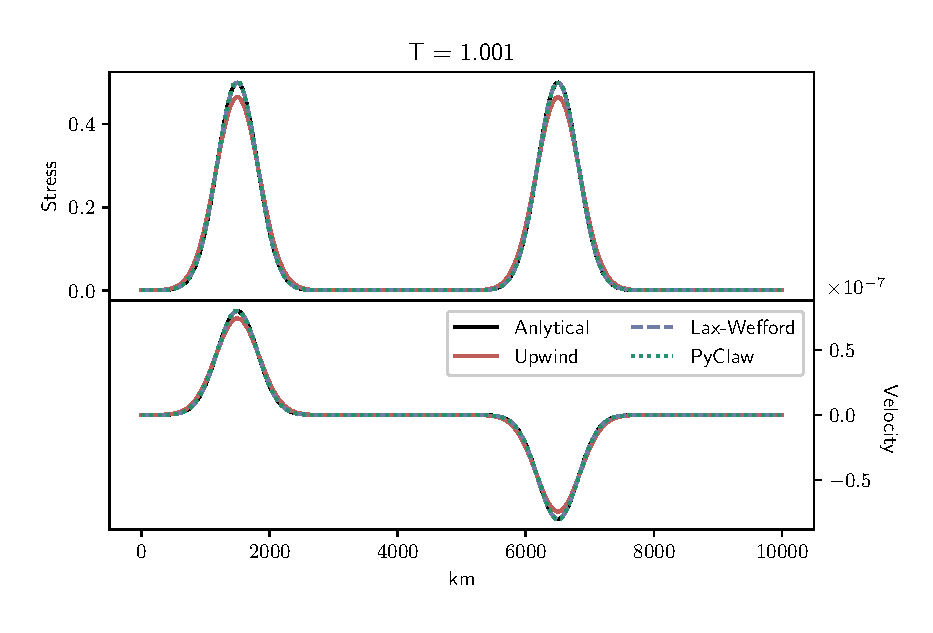
\includegraphics[width=\textwidth]{figs/four_methods.eps}
    \caption{one-dimensional homogeneous elastic wave equation solutions for our three numerical methods plotted against that analytical solution. The PyClaw solution used a Superbee slope limiter. Results are plotted after $\approx$ 1 second of time integration.}
    \label{fig:homo1sec}
\end{figure}

While one second of time integration made the error in the Upwind method apparent, there seemed to be little variability in the Lax-Wefford and Superbee (\texttt{PyClaw}) methods as compared to the analytical solution. To investigate the error in these higher-order methods more, we run the model for 20 seconds of time integration. The code used to run these numerical experiments, along with the figures produced are hosted online as a \href{https://github.com/andrewdnolan/MATH-709-Final-Project}{Github repository}. The repository includes HTML animations of the model run within a Jupyter notebook. Solution vectors at 5, 10, 15, and 20 seconds from the 20 second time integration are plotted in Figure \ref{fig:longrun}. The artificial diffusion from Figure \ref{fig:homo1sec} is even more apparent by five seconds, while there is still strong agreement between the Lax-Wefford and Superbee methods. Note the analytical solution is not plotted in Figure \ref{fig:longrun}, given that I was unable to implement the periodic boundary conditions for the analytical solution. Therefore, we are using the \texttt{PyClaw} solution as our reference which we compare the Upwind and Lax-Wefford solutions against. Note the velocity solution after 10 seconds of time integration in Figure \ref{fig:longrun}. The amplitude of Lax-Wefford scheme is much larger than the than either the Upwind or Superbee solution. There appears to large error when the two waves traveling in opposite directions meet as observed in the velocity solutions at $t=10$ and $t=20$. While the error appears to be large when two waves meet, there does not appear to be much disagreement between the Lax-Wefford and \texttt{PyClaw} solutions after the waves are advected and no longer interfering, as observed in the velocity solution at $t=15$ (Figure \ref{fig:longrun}).  It appears as though the Law-Wefford method does a sufficient job when compared to the Superbee method in the case of the initial condition used here.

\section{Discussion and Conclusion}

Numerical experiments using the elastic wave equation demonstrate large errors in the Upwind method, while there is a modest agreement between the Law-Wefford and Superbee methods, as implemented through \texttt{PyClaw}. While qualitatively there appeared to be agreement between the two methods, a method to quantify the error for each numerical method would have been useful. A method such as the Richardson extrapolation would be a well-suited candidate for such quantification, but was outside the scope of this work. Additionally, the qualitative agreement between the two higher-order methods may be in part due to the initial condition, and therefore waveform being advected, used in this study. The initial condition as represented by Equation \ref{eq:initalcondition} is relative smooth and while there may be steep gradients at points, there are no discontinuities. Therefore, to more robustly test the capabilities of the methods outlined above, one would want to use an end member waveform such as one with discontinuity. Another shortcoming of this study was the efficiency of the code used to run these experiments. Given the nature of the coupled equation and matrix multiplication, the equation was not simply vectorized and therefore solved via nested for loops. We also used explicit methods, as is common practice to hyperbolic systems \cite{leveque_2002}, and therefore could not make use of iterative solvers such as GMRES or the conjugate gradient method. An immediate step to take in the future will be implementing the \texttt{PyClaw} package in parallel as is supported through PETSc.

While the code may not have as efficient as possible and no robust error quantification was done, the work none the less was fruitful. Based on physical intuition and guided by \cite{leveque_2002} we derived conservation laws from which we can formulate the advection equation (Equation \ref{eq:homoadvection}). We then derived the framework of the finite volume method based on numerical approximations of fluxes into and out of our control volume. The sound physical framework on which conservation laws and finite volume methods are derived from has left us with an appreciation for the numerical method. Next, we derived an analytical solution to the one-dimensional elastic wave equation through the method of characteristics. This derivation of an analytical solution demonstrated the significance of the eigendecomposition to physical problems. Having seen material properties such as the shear velocity $C$ and the seismic impedance $Z$ stated in previous courses it was illuminating to see how these material properties are derived. Our derivation of the analytical solution and the decomposition of $A$ also informed our discussion of the Riemann problem. Finally, we conducted the numerical experiment using the first and second-order finite volume methods stated above, and also successfully implemented higher-order solutions through the \texttt{PyClaw} package. The work done here represents a formal introduction to the finite volume method and the \texttt{PyClaw} package from which these methods could be used for genuine scientific inquiry. 

\begin{figure}
    \centering
    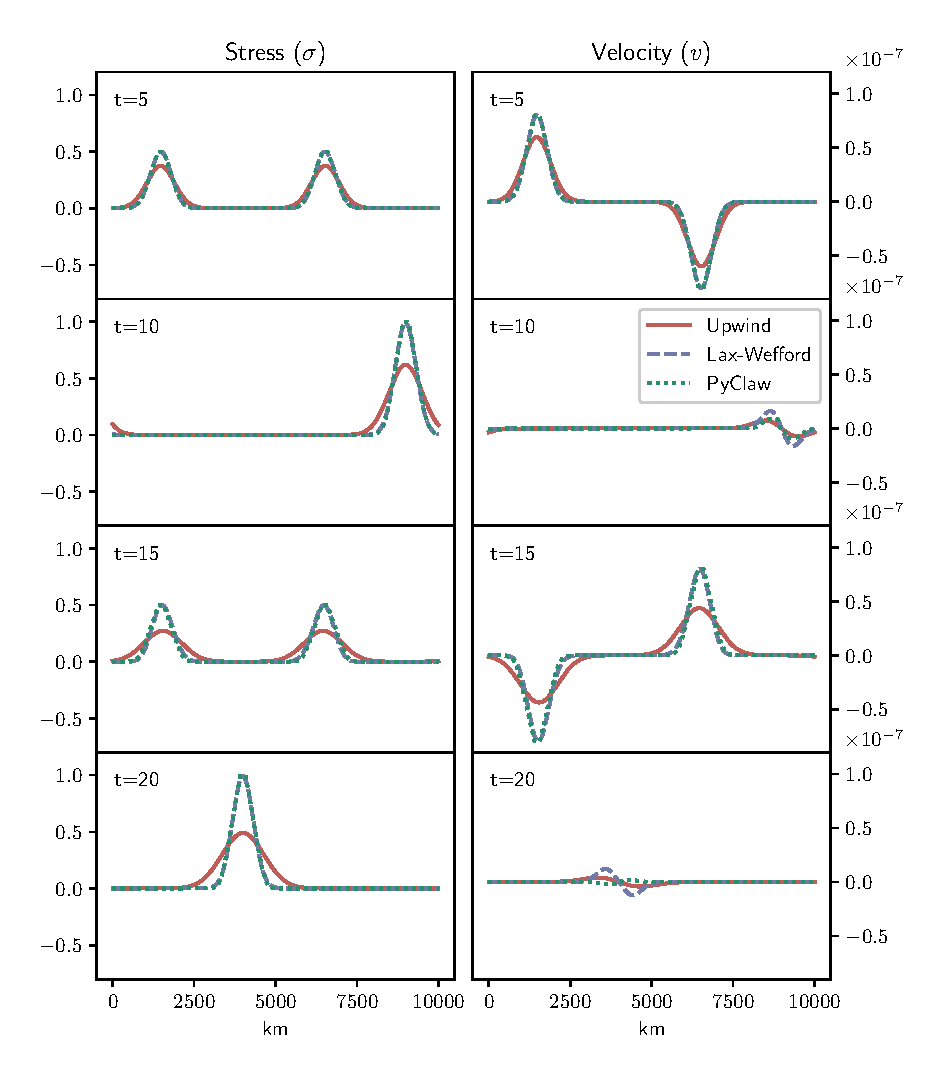
\includegraphics[width=\textwidth]{figs/longrun.eps}
    \caption{Stress and velocity solutions, left and right columns respectively, for the three numerical methods plotted after 5, 10, 15, and 20 seconds of time integration. Note the analytical solution is not plotted. I was not able to implement the periodic boundary condition on the analytical solution and therefore after one full period, the results no longer appropriate to compare our numerical results against. }
    \label{fig:longrun}
\end{figure}
\section*{Supplementary material}
The code used to run these numerical experiments along with annimations of the model runs can be found  \href{https://github.com/andrewdnolan/MATH-709-Final-Project}{here}.

\bibliographystyle{siamplain}
\bibliography{references}
\end{document}
